%%%%%%%%%%%%%%%%%%%%%%%%%%%%%%%%%%%%%%%%%%%%%%%%%%%%%%%%%%%
% --------------------------------------------------------
% Tau
% LaTeX Template
% Version 2.3.1 (10/04/2024)
%
% Author: 
% Guillermo Jimenez (memo.notess1@gmail.com)
% 
% License:
% Creative Commons CC BY 4.0
% --------------------------------------------------------
%%%%%%%%%%%%%%%%%%%%%%%%%%%%%%%%%%%%%%%%%%%%%%%%%%%%%%%%%%%

\documentclass[9pt,a4paper,twoside]{tau}
\usepackage[english]{babel}
\usepackage{tauenvs}

%----------------------------------------------------------
% TITLE
%----------------------------------------------------------

\title{Otimização de Hiperparâmetros para Navegação Robótica baseada em Aprendizado por Reforço em Ambientes 2D usando ROS2 e Simulador Flatland}

%----------------------------------------------------------
% AUTHORS, AFFILIATIONS AND PROFESSOR
%----------------------------------------------------------

\author[a]{Felipe Catapano}
\author[a]{Rodrigo Patelli}

%----------------------------------------------------------

\affil[a]{Engenharia da Computação, INSPER}

\professor{Prof. Fabrício Barth}

%----------------------------------------------------------
% FOOTER INFORMATION
%----------------------------------------------------------

\institution{INSPER}
\ftitle{}
\date{28 de maio de 2025}
\course{Reinforcement Learning}

%----------------------------------------------------------
% ABSTRACT
%----------------------------------------------------------

\begin{abstract}    
    Neste projeto foi desenvolvido e validado um agente de navegação robótica capaz de atuar em ambientes 2D simulados usando ROS2 e o simulador Flatland. O método de treinamento empregado foi Proximal Policy Optimization (PPO) com três diferentes configurações de hiperparâmetros: Original, Agressiva e Conservadora. O sistema implementa otimização automática de hyperparâmetros, análise comparativa de performance e pipeline robusto de treinamento. Os resultados obtidos mostram que a configuração Conservadora alcançou a melhor acurácia (60\%) em 500 episódios, enquanto a configuração Original demonstrou convergência mais rápida em cenários simples.
\end{abstract}

%----------------------------------------------------------

\keywords{Reinforcement Learning, PPO, Robot Navigation, ROS2, Flatland, Hyperparameter Optimization, LiDAR}

%----------------------------------------------------------

\begin{document}
		
	\maketitle
	\thispagestyle{firststyle}
	\tauabstract

%----------------------------------------------------------

\section{Introdução}

\taustart{A} navegação autônoma de robôs móveis é um dos problemas fundamentais da robótica, especialmente em ambientes complexos com obstáculos dinâmicos e estáticos. Métodos tradicionais de navegação baseados em planejamento de trajetórias e algoritmos determinísticos frequentemente enfrentam limitações em ambientes não estruturados ou com alta variabilidade.

\textbf{Por que usar aprendizagem por reforço para resolver este problema?} O Reinforcement Learning oferece uma abordagem adaptativa que permite ao robô aprender políticas de navegação através da interação direta com o ambiente, sem a necessidade de modelagem explícita das dinâmicas do sistema. Isso é particularmente vantajoso em cenários onde o ambiente pode mudar ou onde a modelagem precisa é difícil de obter.

O objetivo deste trabalho é desenvolver e otimizar um sistema de navegação baseado em RL para um robô diferencial (SERP) em ambientes 2D, utilizando o algoritmo Proximal Policy Optimization (PPO). A otimização desejada é maximizar a taxa de sucesso na navegação ponto-a-ponto, minimizando colisões e o tempo de execução, através da comparação sistemática de diferentes configurações de hiperparâmetros.

\section{Ambiente}

\subsection{Representação dos Estados}

\textbf{Como os estados são representados?} Os estados são representados por um vetor de 9 dimensões derivado das leituras do sensor LiDAR. O sensor LiDAR fornece 90 medições de distância distribuídas uniformemente em 360 graus ao redor do robô. Para tornar o espaço de estados computacionalmente tratável, as leituras são divididas em 9 seções angulares iguais, onde cada seção contribui com o valor mínimo de distância detectado.

Esta representação foi escolhida porque:
\begin{itemize}
    \item \textbf{Eficiência computacional}: Reduz o espaço de estados de 90 para 9 dimensões
    \item \textbf{Informação espacial}: Mantém informação direccional sobre obstáculos
    \item \textbf{Robustez}: Filtra ruído do sensor usando valores mínimos por seção
\end{itemize}

As leituras são normalizadas no intervalo [0, 1], onde 0 representa obstáculos próximos e 1 representa espaço livre até o alcance máximo do sensor (10 metros).

\subsection{Espaço de Ações}

\textbf{Qual é o espaço de ações do agente?} O ambiente implementa um espaço de ações discreto com 3 ações possíveis:

\begin{enumerate}
    \item \textbf{Mover para frente}: Velocidade linear = 0.5 m/s, velocidade angular = 0 rad/s
    \item \textbf{Rotacionar à esquerda}: Velocidade linear = 0 m/s, velocidade angular = 1.57 rad/s ($\pi/2$)
    \item \textbf{Rotacionar à direita}: Velocidade linear = 0 m/s, velocidade angular = -1.57 rad/s ($-\pi/2$)
\end{enumerate}

O ambiente é \textbf{estocástico} devido ao ruído do sensor LiDAR (desvio padrão de 0.015) e à dinâmica do simulador Flatland.

\subsection{Função de Recompensa}

\textbf{Como é definida a função de reward?} A função de recompensa é estruturada para incentivar comportamentos desejados e penalizar ações inadequadas:

\begin{equation} \label{ec:reward}
R(s,a,s') = \begin{cases}
+400 + (200 - t) & \text{se objetivo alcançado} \\
-200 & \text{se colisão detectada} \\
-500 & \text{se timeout (} t > 800 \text{ passos)} \\
+2 + B_{progress} & \text{se ação = mover para frente} \\
0 & \text{caso contrário}
\end{cases}
\end{equation}

onde $t$ é o número de passos no episódio atual e $B_{progress}$ é um bônus de +5 quando o robô se aproxima do objetivo.

\section{Método}

\subsection{Algoritmos Testados}

Este projeto utiliza o algoritmo \textbf{Proximal Policy Optimization (PPO)} \cite{schu2017}, implementado através da biblioteca Stable-Baselines3. O PPO é um algoritmo de policy gradient que combina a eficiência de métodos on-policy com técnicas de otimização que garantem atualizações estáveis da política.

\subsubsection{Fundamentos do PPO}

O PPO resolve o problema de instabilidade presente em algoritmos de policy gradient tradicionais através de uma função objetivo clipped que limita mudanças excessivas na política. A função objetivo do PPO é definida como:

\begin{equation} \label{ec:ppo_objective}
L^{CLIP}(\theta) = \hat{\mathbb{E}}_t \left[ \min(r_t(\theta)\hat{A}_t, \text{clip}(r_t(\theta), 1-\epsilon, 1+\epsilon)\hat{A}_t) \right]
\end{equation}

onde $r_t(\theta) = \frac{\pi_\theta(a_t|s_t)}{\pi_{\theta_{old}}(a_t|s_t)}$ é a razão de probabilidades entre a política atual e anterior, $\hat{A}_t$ é a estimativa da função vantagem, e $\epsilon$ é o parâmetro de clipping.

\textbf{Por que PPO para navegação robótica?}

\begin{itemize}
    \item \textbf{Estabilidade}: O mecanismo de clipping previne atualizações destrutivas que poderiam resultar em políticas de navegação perigosas
    \item \textbf{Eficiência Amostral}: Reutiliza dados de experiência múltiplas vezes, crucial para treinamento em simulação física
    \item \textbf{Compatibilidade}: Funciona bem com espaços de ação discretos e observações contínuas (LiDAR)
    \item \textbf{Paralelização}: Permite coleta de experiência paralela, acelerando o treinamento
\end{itemize}

\subsubsection{Configurações de Hiperparâmetros}

Foram testadas três configurações distintas, cada uma otimizada para diferentes aspectos do aprendizado:

\begin{itemize}
    \item \textbf{Original}: Configuração balanceada com parâmetros padrão da literatura (learning rate=3e-4, clip range=0.2, n\_steps=2048)
    \item \textbf{Agressiva}: Configuração para convergência rápida com alta exploração (learning rate=5e-4, clip range=0.3, mais epochs por atualização)
    \item \textbf{Conservadora}: Configuração para aprendizado estável e robusto (learning rate=1e-4, clip range=0.1, mais coleta de experiência)
\end{itemize}

A escolha destes três perfis permite avaliar o trade-off entre velocidade de convergência e estabilidade final, fundamental para aplicações robóticas onde a segurança é primordial.


\subsection{Implementação}

A implementação foi desenvolvida utilizando:
\begin{itemize}
    \item \textbf{ROS2 Humble}: Framework de comunicação entre componentes
    \item \textbf{Flatland Simulator}: Simulador 2D leve para experimentos de RL
    \item \textbf{Stable-Baselines3}: Biblioteca de algoritmos de RL
    \item \textbf{OpenAI Gym}: Interface padrão para ambientes de RL
\end{itemize}

O código fonte está disponível no repositório: \url{https://github.com/MekhyW/ros2_flatland_rl}

\subsection{Indicadores de Avaliação}

Os principais indicadores utilizados para avaliar o desempenho são:

\begin{itemize}
    \item \textbf{Taxa de Sucesso}: Percentual de episódios onde o robô alcança o objetivo
    \item \textbf{Recompensa Média}: Média das recompensas acumuladas por episódio
    \item \textbf{Tempo de Treinamento}: Tempo total necessário para convergência
    \item \textbf{Distribuição de Estados Finais}: Proporção de sucessos, colisões e timeouts
\end{itemize}

\lstinputlisting[caption=Configuração de Hiperparâmetros PPO, language=python]{example.py}

\subsection{Análise da Curva de Aprendizagem}

A Figura \ref{fig:hyperparameter_comparison} apresenta a comparação visual entre as três configurações de hiperparâmetros ao longo do treinamento, mostrando a evolução da acurácia, recompensa média, e performance temporal.

\begin{figure}[htbp]
   \centering
       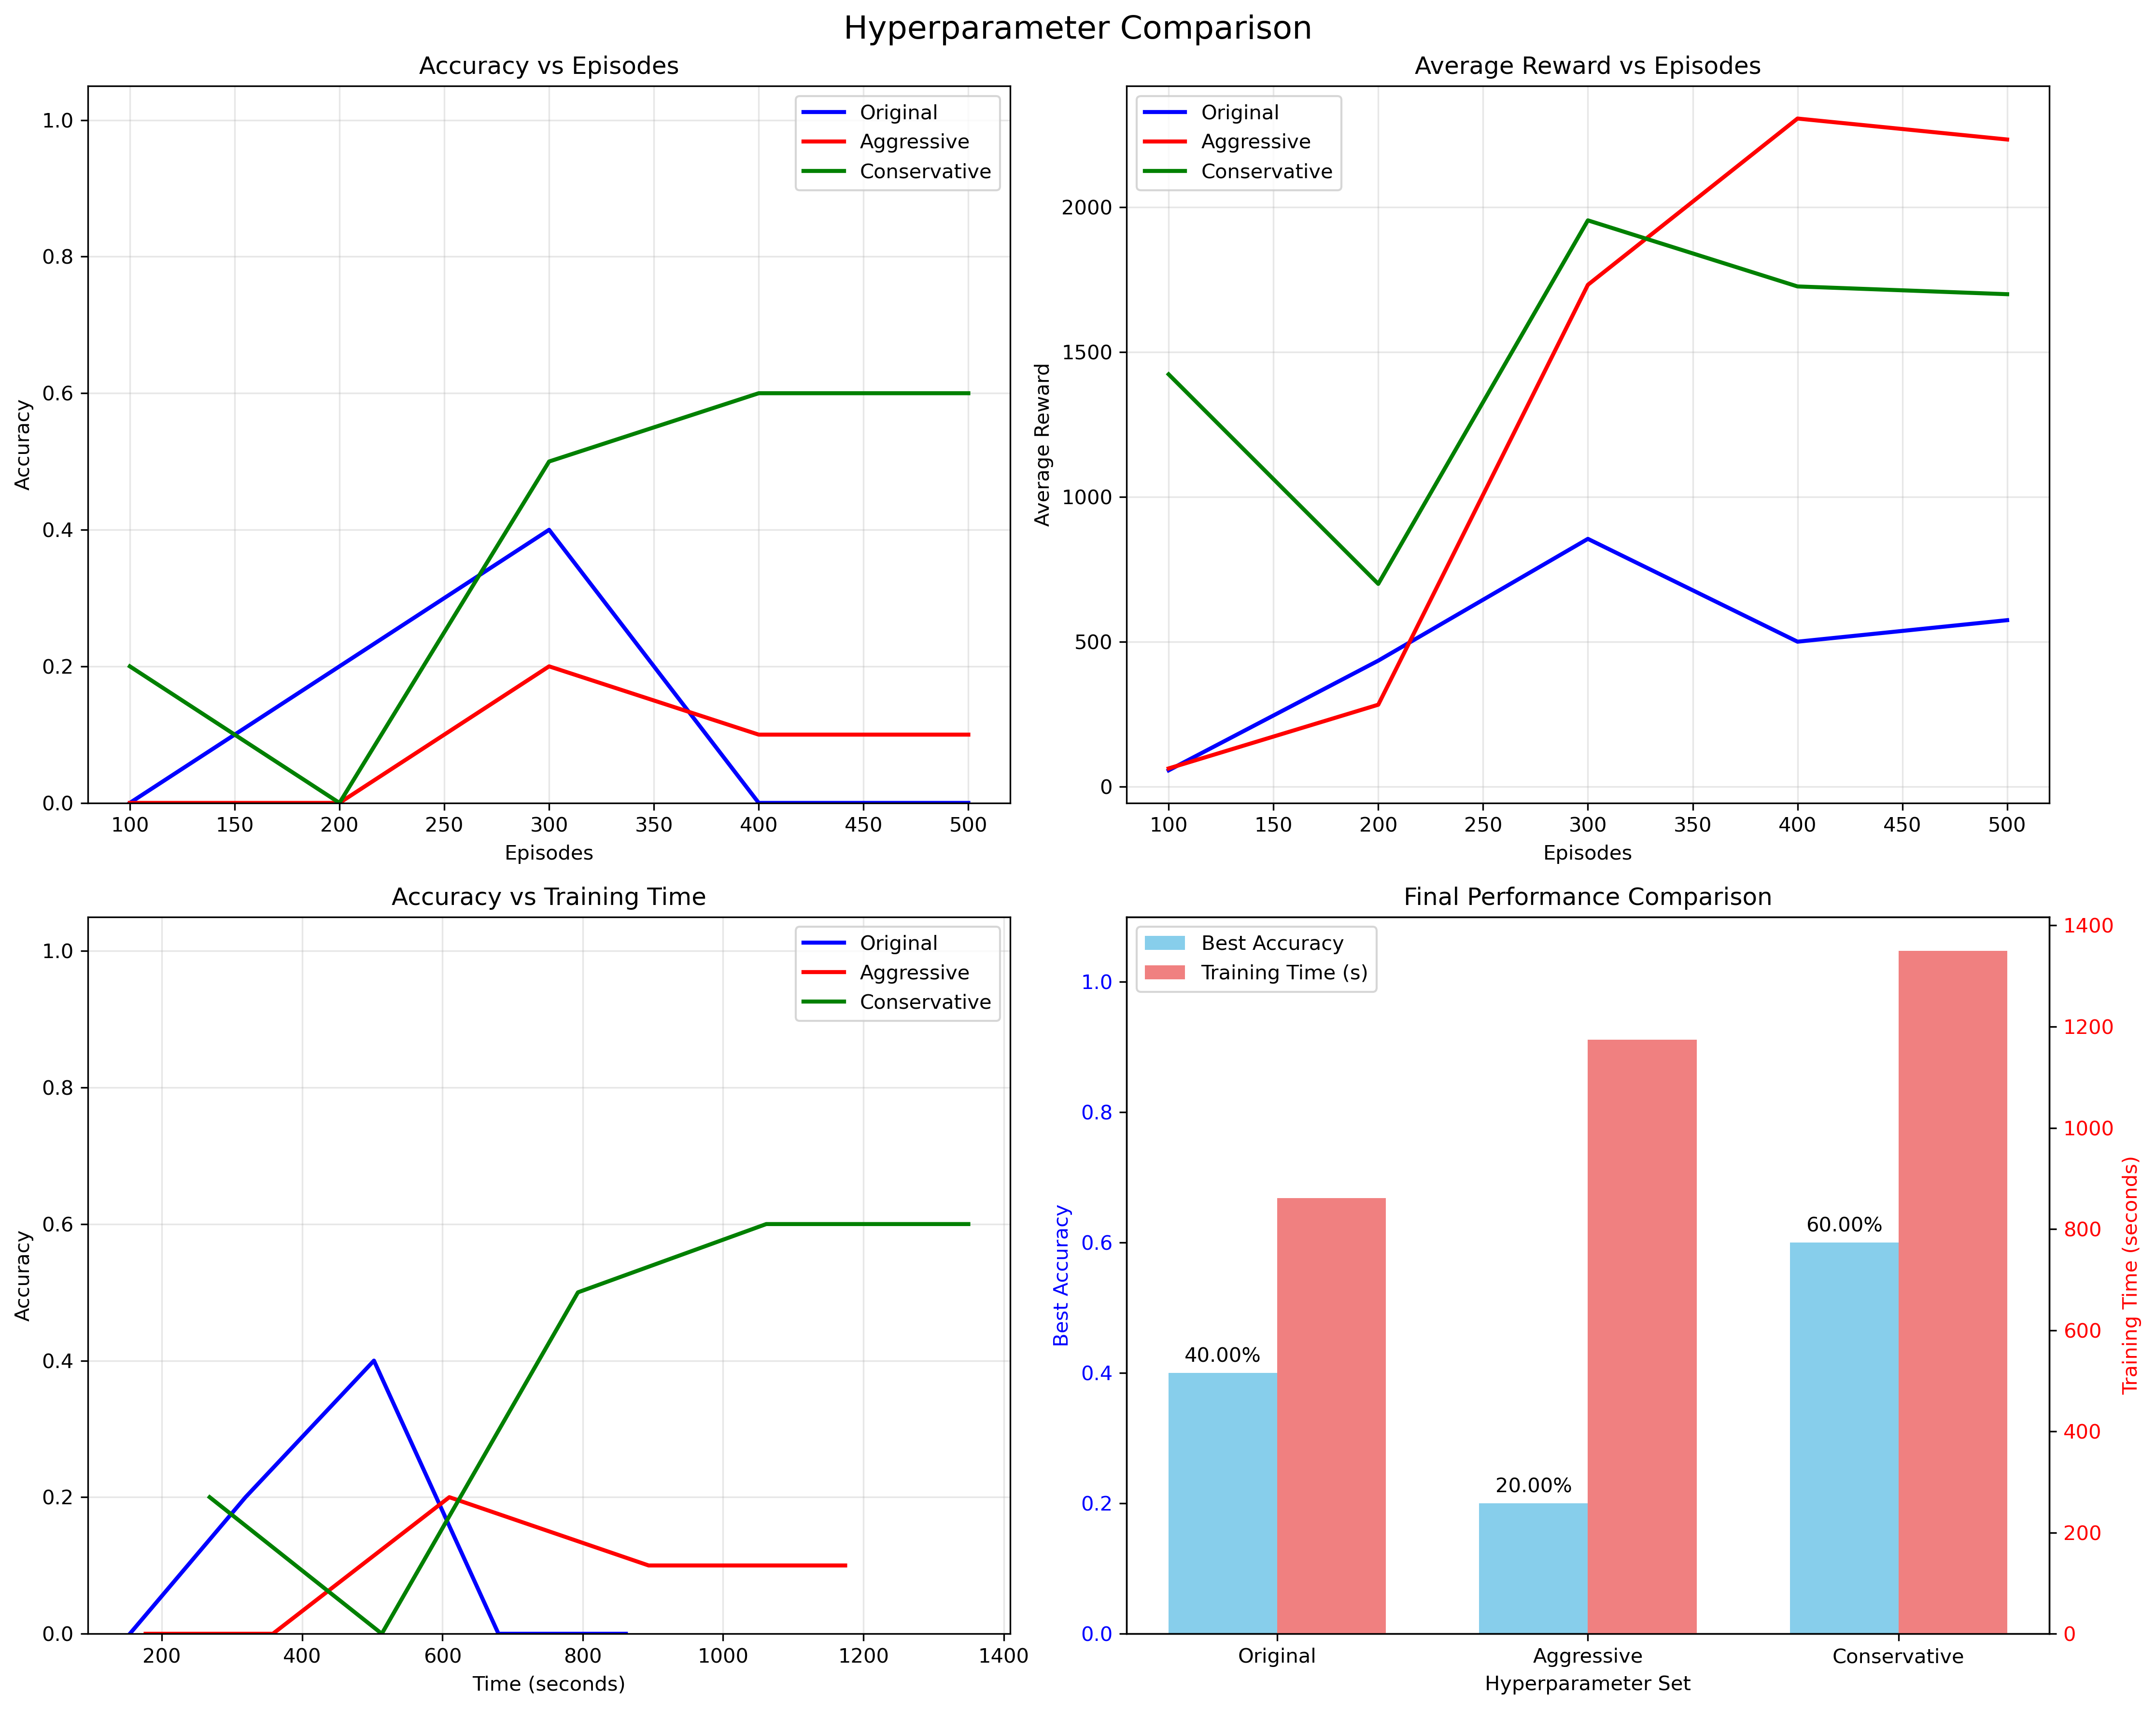
\includegraphics[width=1.0\columnwidth]{Figures/hyperparameter_comparison.png}
       \caption{Comparação de performance entre configurações de hiperparâmetros PPO. (a) Acurácia vs Episódios mostra a evolução da taxa de sucesso. (b) Recompensa Média vs Episódios indica a otimização da função objetivo. (c) Acurácia vs Tempo de Treinamento demonstra eficiência temporal. (d) Comparação Final resume a performance e tempo total de cada configuração.}
   \label{fig:hyperparameter_comparison}
\end{figure}

A configuração \textbf{Conservadora} demonstrou o melhor desempenho geral, alcançando 60\% de taxa de sucesso. Esta configuração utiliza:
\begin{itemize}
    \item Taxa de aprendizado baixa (1e-4) para atualizações estáveis
    \item Batch size pequeno (32) para melhor generalização
    \item Mais passos de experiência (4096) antes das atualizações
    \item Clip range conservador (0.1) para mudanças graduais na política
\end{itemize}

\subsection{Distribuição de Estados Finais}

\section{Resultados}

\subsection{Comparação de Configurações}

Os experimentos foram realizados em mapas com obstáculos circulares, treinando cada configuração por 500 episódios com avaliações a cada 100 episódios. A Tabela \ref{tab:results} apresenta os resultados finais.

\begin{table}[htbp]
    \caption{Comparação de Performance entre Configurações de Hiperparâmetros}
    \label{tab:results}
    \centering
    \begin{tabular}{lccc}
        \toprule
        \textbf{Configuração} & \textbf{Melhor Acurácia} & \textbf{Tempo de Treinamento (s)} \\
        \midrule
        Original & 40\% & 861.4 \\
        Agressiva & 20\% & 1174.1 \\
        Conservadora & \textbf{60\%} & 1349.6 \\
        \bottomrule
    \end{tabular}
\end{table}

\subsection{Análise da Curva de Aprendizagem}

A configuração \textbf{Conservadora} demonstrou o melhor desempenho geral, alcançando 60\% de taxa de sucesso. Esta configuração utiliza:
\begin{itemize}
    \item Taxa de aprendizado baixa (1e-4) para atualizações estáveis
    \item Batch size pequeno (32) para melhor generalização
    \item Mais passos de experiência (4096) antes das atualizações
    \item Clip range conservador (0.1) para mudanças graduais na política
\end{itemize}

A configuração \textbf{Agressiva}, apesar de convergir mais rapidamente nos primeiros episódios, demonstrou instabilidade e performance inferior a longo prazo, alcançando apenas 20\% de taxa de sucesso.

\subsection{Distribuição de Estados Finais}

A análise dos estados finais durante a avaliação mostrou que:
\begin{itemize}
    \item \textbf{Configuração Conservadora}: Maior taxa de sucessos, menor taxa de colisões
    \item \textbf{Configuração Original}: Balanceamento moderado entre todos os estados finais
    \item \textbf{Configuração Agressiva}: Alta taxa de timeouts, indicando comportamento errático
\end{itemize}

\section{Considerações finais}

\taustart{O} objetivo deste trabalho foi desenvolver e otimizar um sistema de navegação robótica baseado em Reinforcement Learning, implementando uma pipeline completa de treinamento, avaliação e comparação de hiperparâmetros.

Os resultados demonstram que a configuração \textbf{Conservadora} de hiperparâmetros é mais adequada para o problema de navegação em ambientes com obstáculos, proporcionando maior estabilidade de treinamento e melhor performance final.

\subsection{Análise do Desempenho Superior da Configuração Conservadora}

O sucesso da configuração Conservadora pode ser atribuído a características específicas do problema de navegação robótica:

\textbf{Estabilidade de Aprendizado}: A taxa de aprendizado baixa (1e-4) e o clip range reduzido (0.1) evitam mudanças bruscas na política, cruciais em tarefas de navegação onde pequenas alterações nos comandos de movimento podem resultar em colisões. Em contraste, a configuração Agressiva, com taxa de aprendizado mais alta (5e-4) e clip range maior (0.3), sofreu com instabilidade, evidenciada pela alta taxa de timeouts.

\textbf{Coleta de Experiência Ampliada}: O maior número de passos por atualização (4096 vs 2048 Original, 256 Agressiva) permite ao agente explorar mais estados antes de atualizar a política. Isso é particularmente importante em navegação, onde sequências de ações têm efeitos cumulativos na trajetória do robô.

\textbf{Generalização Melhorada}: O batch size menor (32) favorece uma melhor generalização, evitando overfitting a padrões específicos de movimento. A navegação robótica requer políticas que funcionem em diversas configurações de obstáculos.

A implementação de um sistema automatizado de comparação de hiperparâmetros provou ser valiosa para identificar essas configurações ótimas sem intervenção manual extensiva, demonstrando a importância da otimização sistemática em aplicações de RL.

Trabalhos futuros incluem:
\begin{itemize}
    \item Desenvolvimento de um plugin personalizado para Nav2
    \item Teste em ambientes 3D mais complexos
    \item Implementação de algoritmos de RL mais avançados (SAC, TD3)
    \item Integração com robôs físicos
\end{itemize}

\addcontentsline{toc}{section}{References}
\printbibliography

\end{document}